%auto-ignore



\section{BERT}
\label{sec:bert}

% BERT: what is pretraining and what is fine tuning at high level
본 절에서는 BERT와 그 상세 구현을 소개한다. 저자들의 프레임워크는 두 단계로 구성된다 — \emph{사전학습(pre-training)}과 \emph{파인튜닝(fine-tuning)}.
사전학습 동안 모델은 서로 다른 사전학습 과제 위에서 비라벨 데이터로 학습된다.
파인튜닝에서는 BERT 모델을 먼저 사전학습된 파라미터로 초기화한 뒤, 다운스트림 과제의 라벨 데이터를 이용해 모든 파라미터를 파인튜닝한다.
다운스트림 과제마다 별도의 파인튜닝된 모델이 만들어지지만, 모두 같은 사전학습 파라미터로 초기화된다. 그림~\ref{fig:bert_overall}의 질의응답 예시가 본 절을 관통하는 진행 예시 역할을 한다.

BERT의 두드러진 특징은 서로 다른 과제에 걸쳐 통일된 아키텍처를 사용한다는 점이다.
사전학습 아키텍처와 최종 다운스트림 아키텍처 사이에는 차이가 거의 없다.

\paragraph{모델 아키텍처}
BERT의 모델 아키텍처는 \citet{vaswani-etal:2017:_atten}에 기술되고 {\tt tensor2tensor} 라이브러리에 공개된 원본 구현에 기반한 다층 양방향 트랜스포머 인코더이다.\footnote{https://github.com/tensorflow/tensor2tensor} 트랜스포머의 사용이 일반화되었고 저자들의 구현이 원본과 거의 동일하기 때문에, 모델 아키텍처에 대한 상세 배경 설명은 생략하고 \citet{vaswani-etal:2017:_atten}이나 ``The Annotated Transformer''\footnote{http://nlp.seas.harvard.edu/2018/04/03/attention.html} 같은 훌륭한 가이드를 참고하기를 권한다.

본 연구에서, 저자들은 트랜스포머 블록의 수(즉, 층수)를 $L$, 히든 크기를 $H$, 셀프 어텐션 헤드 수를 $A$로 표기한다.\footnote{모든 경우 피드포워드/필터 크기는 $4H$로 설정한다(즉, $H=768$일 때 3072, $H=1024$일 때 4096).} 저자들은 주로 두 가지 모델 크기에 대한 결과를 보고한다 — {\bf \bertbase} ($L=12$, $H=768$, $A=12$, 총 파라미터 110M)와 {\bf \bertlarge} ($L=24$, $H=1024$, $A=16$, 총 파라미터 340M).

\bertbase는 비교 목적으로 OpenAI GPT와 같은 모델 크기를 갖도록 선택되었다. 그러나 결정적으로, BERT 트랜스포머는 양방향 셀프 어텐션을 사용하는 반면, GPT 트랜스포머는 모든 토큰이 자기 왼쪽 맥락에만 어텐션할 수 있는 제약된(셀프) 어텐션을 사용한다.\footnote{문헌에서 양방향 트랜스포머를 흔히 ``트랜스포머 인코더''라고 부르고, 좌측 맥락만 보는 버전은 텍스트 생성에 사용될 수 있어 ``트랜스포머 디코더''로 부른다는 점에 유의한다.}


\paragraph{입력/출력 표현} % Claim we shared the structures
BERT가 다양한 다운스트림 과제를 다룰 수 있게 하기 위해,
저자들의 입력 표현은 단일 문장과 한 쌍의 문장(예: $\langle$질문, 답변$\rangle$)을 모두 하나의 토큰 시퀀스 안에서 모호함 없이 표현할 수 있다. 본 연구에서 ``문장(sentence)''은 실제 언어학적 문장이 아니라 임의의 연속 텍스트 구간을 의미할 수 있다. ``시퀀스(sequence)''는 BERT의 입력 토큰 시퀀스를 가리키며, 단일 문장이거나 두 문장이 묶인 형태일 수 있다.

저자들은 30,000 토큰 어휘의 WordPiece 임베딩을 사용한다~\cite{wu-etal:2016:_googl}.
%We denote split word pieces with {\tt \#\#}. We use learned positional embeddings with supported sequence lengths up to 512 tokens.
모든 시퀀스의 첫 번째 토큰은 항상 특수 분류 토큰({\tt [CLS]})이다. 이 토큰에 해당하는 최종 은닉 상태는 분류 과제를 위한 시퀀스 전체의 집계 표현으로 사용된다.
%For non-classification tasks, this vector is ignored.
문장 쌍은 하나의 시퀀스로 묶인다. 저자들은 두 가지 방식으로 두 문장을 구분한다. 첫째, 특수 토큰({\tt [SEP]})으로 두 문장을 분리한다. 둘째, 모든 토큰에 그 토큰이 문장 {\tt A}에 속하는지 문장 {\tt B}에 속하는지를 가리키는 학습 가능한 임베딩을 더한다.
그림~\ref{fig:bert_overall}에서 보이듯, 저자들은 입력 임베딩을 $E$로, 특수 {\tt [CLS]} 토큰의 최종 은닉 벡터를 $C \in \mathbb{R}^{H}$로, $i$번째 입력 토큰의 최종 은닉 벡터를 $T_i \in \mathbb{R}^H$로 표기한다.

주어진 토큰의 입력 표현은 그에 대응하는 토큰·세그먼트·위치 임베딩을 합산해 만든다.
이 구성의 시각화는 그림~\ref{fig:input_embeddings}에서 볼 수 있다.

\begin{figure*}[ht]
\begin{center}
\hspace{-0.2in}
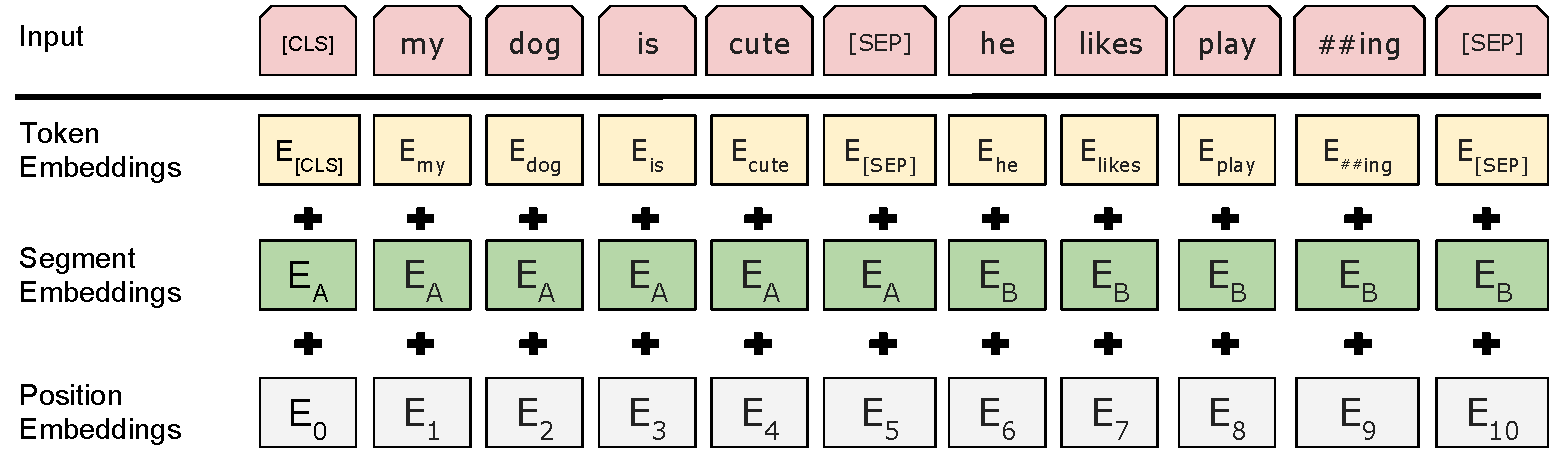
\includegraphics[width=0.85\textwidth]{Input_Emebeddings.pdf}
\end{center}
\caption{BERT 입력 표현. 입력 임베딩은 토큰 임베딩, 세그먼테이션 임베딩, 위치 임베딩의 합이다.}
\label{fig:input_embeddings}
\end{figure*}


%In the subsequent model descriptions,


\subsection{BERT 사전학습}
\label{sec:pretraining_tasks}

\citet{peters-etal:2018:_deep}이나 \citet{radford-etal:2018}과 달리, 저자들은 BERT를 사전학습할 때 전통적인 좌→우나 우→좌 언어모델을 사용하지 않는다. 대신, 본 절에서 설명하는 두 개의 비지도 과제로 BERT를 사전학습한다. 이 단계는 그림~\ref{fig:bert_overall}의 왼쪽 부분에 묘사되어 있다.

%\noindent\textbf{Task \#1: Masked LM}
\paragraph{과제 \#1: 마스킹 LM}
직관적으로, 깊은 양방향 모델이 좌→우 모델이나 좌→우/우→좌 모델의 얕은 결합보다 엄격하게 더 강력하다고 믿는 것은 합리적이다. 그러나 표준 조건부 언어모델은 좌→우 \emph{또는} 우→좌로만 학습될 수 있다 — 양방향 조건부 분포는 각 단어가 간접적으로 ``자기 자신을 보게'' 만들어, 다층 맥락에서 모델이 목표 단어를 자명하게 예측해 버리기 때문이다.

깊은 양방향 표현을 학습하기 위해, 저자들은 입력 토큰의 일정 비율을 무작위로 마스킹하고 그 마스킹된 토큰을 예측한다. 저자들은 이 절차를 ``마스킹 LM''(MLM)이라 부르며, 문헌에서는 흔히 \emph{Cloze} 과제로도 불린다~\cite{taylor:1953:_cloze}. 이 경우, 마스크 토큰에 대응하는 최종 은닉 벡터는 표준 LM처럼 어휘 위 출력 소프트맥스에 입력된다. 모든 실험에서 저자들은 각 시퀀스의 모든 WordPiece 토큰의 15\,\%를 무작위로 마스킹한다. 잡음제거 오토인코더~\cite{vincent:2008}와 달리, 입력 전체를 복원하는 대신 마스킹된 단어만 예측한다.
%Unlike \citet{melamud2016context2vec}, we mask multiple input tokens at the same time and train a deep bi-directional encoder instead of a top-level combination of left and right context encoders. In addition, we use additional token-level objectives more similar to ones in denoising auto-encoders and auto-encoders (see last two prediction tasks in the list below).

이렇게 하면 양방향 사전학습 모델을 얻을 수 있지만, 단점은 \emph{사전학습과 파인튜닝 사이의 불일치}가 생긴다는 점이다 — {\tt [MASK]} 토큰은 파인튜닝에는 등장하지 않기 때문이다. 이를 완화하기 위해, ``마스킹된'' 단어를 항상 실제 {\tt [MASK]} 토큰으로 바꾸지는 않는다. 학습 데이터 생성기는 예측 대상으로 토큰 위치의 15\,\%를 무작위로 선택한다. $i$번째 토큰이 선택되면, 80\,\% 확률로 (1) {\tt [MASK]} 토큰으로, 10\,\% 확률로 (2) 임의의 토큰으로, 10\,\% 확률로 (3) 변경 없이 원래의 $i$번째 토큰으로 둔다. 그 뒤 $T_i$가 교차 엔트로피 손실로 원본 토큰을 예측하는 데 사용된다.
이 절차의 변형들은 부록~\ref{appendix:sec:different_masks}에서 비교한다.
\vspace{.2cm}

%\noindent\textbf{Task \#2: Next Sentence Prediction (NSP)}
\paragraph{과제 \#2: 다음 문장 예측 (NSP)}
질의응답(QA)이나 자연어 추론(NLI) 같은 많은 중요한 다운스트림 과제는 두 문장 사이의 \emph{관계} 이해에 기반하는데, 이는 언어모델링이 직접 포착하지는 못한다. 문장 간 관계를 이해하는 모델을 학습하기 위해, 저자들은 어떤 단일 언어 코퍼스에서도 손쉽게 생성할 수 있는 이진화된 \emph{다음 문장 예측} 과제로 사전학습한다. 구체적으로, 각 사전학습 예시의 문장 {\tt A}와 {\tt B}를 고를 때, 50\,\% 확률로 {\tt B}는 {\tt A} 뒤에 실제로 따라오는 문장이며({\tt {\small IsNext}}로 라벨링), 50\,\% 확률로 코퍼스에서 무작위로 뽑은 문장이다({\tt {\small NotNext}}로 라벨링).
%We choose the {\tt {\small NotNext}} sentences completely at random.
그림~\ref{fig:bert_overall}에서 보이듯, $C$는 다음 문장 예측(NSP)에 사용된다.\footnote{최종 모델은 NSP에서 97\,\%--98\,\% 정확도를 달성한다.} 단순함에도 불구하고, 본 과제로 사전학습하는 것이 QA와 NLI 모두에 매우 유익함을 \S\ref{sec:task_ablation}에서 보인다.
\footnote{$C$ 벡터는 NSP로 학습된 것이므로 파인튜닝 없이는 의미 있는 문장 표현이 아니다.}
NSP 과제는 \citet{DBLP:journals/corr/JerniteBS17}과 \citet{logeswaran2018an}에서 사용된 표현 학습 목적함수와 밀접하게 관련된다. 다만 기존 연구는 문장 임베딩만 다운스트림 과제로 전이한 반면, BERT는 모든 파라미터를 전이해 최종 과제 모델 파라미터를 초기화한다.



\vspace{.3cm}
\noindent\textbf{사전학습 데이터}
사전학습 절차는 언어모델 사전학습에 관한 기존 문헌을 대체로 따른다. 사전학습 코퍼스로는 BooksCorpus(800M 단어)~\cite{zhu:2015}와 영어 Wikipedia(2,500M 단어)를 사용한다. Wikipedia에서는 본문만 추출하고 목록·표·헤더는 무시한다. Billion Word Benchmark~\cite{chelba-etal:2013:_one} 같은 문장 단위로 섞인 코퍼스가 아니라 \emph{문서 단위 코퍼스}를 사용하는 것이 결정적이다 — 그래야 길고 연속적인 시퀀스를 추출할 수 있기 때문이다.

\subsection{BERT 파인튜닝}
\label{sec:finetuning_procedure}

파인튜닝은 직관적이다. 트랜스포머의 셀프 어텐션 메커니즘은, 단일 텍스트든 텍스트 쌍이든 BERT가 입력과 출력만 적절히 교체하는 것만으로 다양한 다운스트림 과제를 모델링할 수 있게 해 주기 때문이다.
텍스트 쌍이 관여하는 응용에서 흔한 패턴은~\newcite{parikh-etal:2016, bidaf}처럼 두 텍스트를 독립적으로 인코딩한 뒤 양방향 교차 어텐션을 적용하는 것이다. BERT는 이를 셀프 어텐션 메커니즘으로 통일한다 — 두 텍스트를 이은 시퀀스를 셀프 어텐션으로 인코딩하는 것 자체가 두 문장 간의 \emph{양방향} 교차 어텐션을 효과적으로 포함하기 때문이다.


각 과제에 대해, 저자들은 과제별 입력과 출력을 단순히 BERT에 꽂아 넣고 모든 파라미터를 엔드-투-엔드로 파인튜닝한다.
%
입력 측면에서, 사전학습의 문장 {\tt A}와 문장 {\tt B}는 (1) 패러프레이즈에서의 문장 쌍, (2) 함의(entailment)에서의 가설-전제 쌍, (3) 질의응답에서의 질문-본문 쌍, (4) 텍스트 분류나 시퀀스 태깅에서의 텍스트-$\varnothing$ 퇴화 쌍에 대응된다. 출력 측면에서, 토큰 표현은 시퀀스 태깅이나 질의응답 같은 토큰 수준 과제의 출력 층에 입력되고, {\tt [CLS]} 표현은 함의나 감성 분석 같은 분류 과제의 출력 층에 입력된다.


사전학습에 비해 파인튜닝은 상대적으로 저렴하다. 본 논문의 모든 결과는 동일한 사전학습 모델에서 출발해, 단일 Cloud TPU에서 최대 1시간 안에, 또는 GPU에서 몇 시간 안에 재현할 수 있다.\footnote{예컨대, BERT SQuAD 모델은 단일 Cloud TPU에서 약 30분 만에 학습되어 Dev F1 91.0\,\%를 달성한다.}
과제별 세부 사항은 \S\ref{sec:experiments}의 해당 소절에서 기술하며, 더 자세한 내용은 부록~\ref{appendix:sec:fine_tune_details_and_figures}에서 다룬다.


\eat{The standard pattern in many NLP models is to independently encode text pairs before apply bidirectional cross attention, such as ~\newcite{parikh-etal:2016, bidaf}. BERT instead leverages the self-attention mechanism in the Transformer to unify these two stages. Encoding with self-attention is performed jointly with \emph{iterative} and \emph{bidirectional} cross attention.
Therefore, many downstream tasks---whether they involve single text or text pairs---can be modeled by simply swapping out the appropriate inputs and outputs.

At the input, sentence {\tt A} and sentence {\tt B} from pre-training are analogous to (1) sentence pairs in paraphrasing, (2) hypothesis-premise pairs in entailment, (3) question-passage pairs in question answering, and (4) a degenerate text-$\varnothing$ pair in text classification or sequence tagging. At the output, the token representations are fed into an output layer for token-level tasks, such as sequence tagging or question answering, and the {\tt [CLS]} representation is fed into an output layer for classification, such as entailment or sentiment analysis.

During the fine-tuning stage, we simply plug in the task-specific inputs and outputs into BERT and fine-tune all the parameters end-to-end. We describe the task-specific details in the corresponding subsections of Section~\ref{sec:experiments}. In-depth task specific design figures are also shown in Appendix~\ref{appendix:sec:fine_tune_details_and_figures}.
}

\eat{
\vspace{.3cm}
\noindent\textbf{Cross-attention}
BERT is designed such that it does not distinguish between self-attention used within a single sequence and cross-attention used between multiple sequences. Cross-attention between
question and passage has been shown to be important for question-answering~\cite{bidaf}, where they cross
attend question and passage for two times.
When fine-tuning a twelve-layer BERT for question answering, the question and passage will cross attend to each other for {\em twelve} times given that question and passage are packed into a single input sequence
\emph{iteratively}. Moreover, the parameters for cross-attention are pretrained. The iterative attention also happened in OpenAI GPT, but
the second sequence cannot attend to the first sequence due to the unidirectionality constraint.
}
